% tikz_labelled.tex -- the two schematics of Theorem 2.17 (Section 2.8), drawn in TikZ.
%   (a) The share fr: the section of B(sqrt(3/2)) by the hyperplane of a centre at
%       height tau is a ball of dimension three and radius rho = (3/2 - tau^2)^(1/2);
%       the hyperplane of a second centre cuts it in a plane at signed distance
%       q rho from its centre, and the cap beyond that plane is the share
%       fr = (1 - q)^2 (2 + q)/4 of the section.  Orthographic, q = 0.35.
%   (b) The three ranges of the largest inner product t of three directions in the
%       proof, with what settles each; not to scale.
% Build:  pdflatex tikz_labelled.tex && pdftoppm -r 500 -png -singlefile tikz_labelled.pdf ../figures/fig_tikz_labelled
\documentclass[border=4pt]{standalone}
\usepackage{tikz}
\usetikzlibrary{calc,arrows.meta,positioning}
\usepackage[T1]{fontenc}
\usepackage{lmodern}
\usepackage{amsmath}
\definecolor{cblue}{HTML}{2A78D6}
\definecolor{corange}{HTML}{EB6834}
\definecolor{caqua}{HTML}{1BAF7A}
\definecolor{cviolet}{HTML}{4A3AA7}
\definecolor{cink}{HTML}{0B0B0B}
\definecolor{cink2}{HTML}{52514E}
\definecolor{cink3}{HTML}{8B8A85}
\definecolor{cpanel}{HTML}{F4F3EF}
\begin{document}
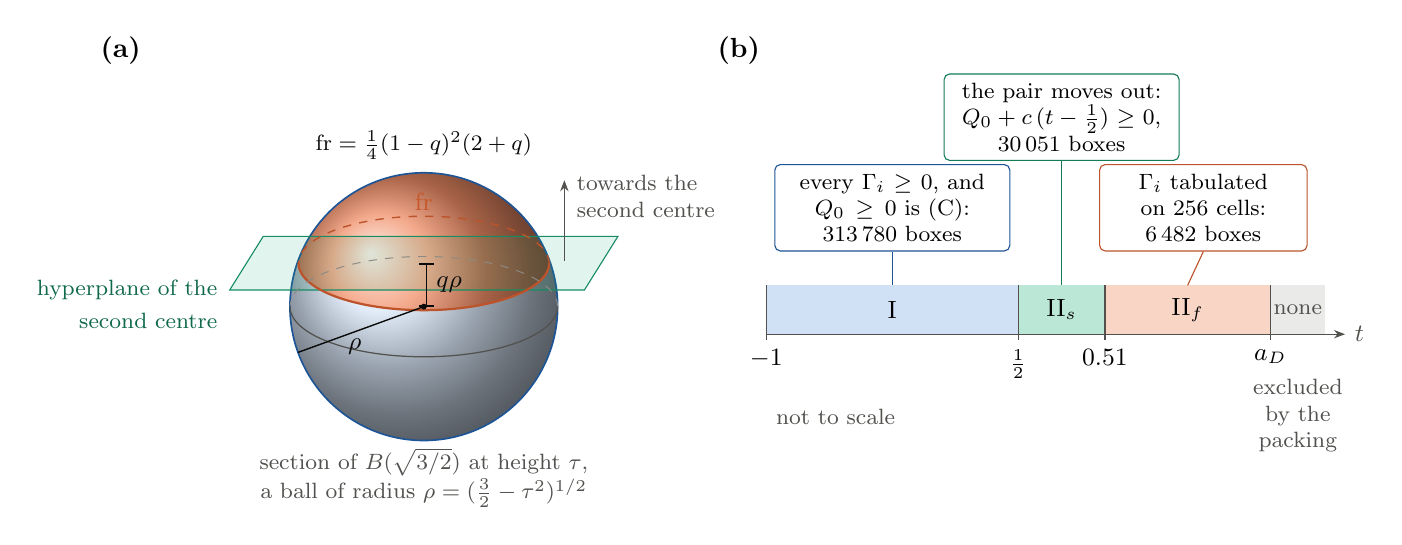
\begin{tikzpicture}[font=\small]
%% ------------------------------------------------------------------ (a)
\begin{scope}[scale=1.7]
  % orthographic view from elevation e: (x, y, z) -> (x, z cos e + y sin e)
  \pgfmathsetmacro{\e}{22}
  \pgfmathsetmacro{\q}{0.35}
  \pgfmathsetmacro{\rz}{sqrt(1-\q*\q)}          % radius of the cutting circle (rho = 1)
  \pgfmathsetmacro{\yc}{\q*cos(\e)}             % screen height of its centre
  \pgfmathsetmacro{\ry}{\rz*sin(\e)}            % vertical semi-axis of its image
  % the section ball
  \shade[ball color=cblue!18] (0,0) circle (1);
  % the cap beyond the plane: inside the ball, above the front arc of the circle
  \begin{scope}
    \clip (0,0) circle (1);
    \clip (-\rz,\yc) arc[start angle=180, end angle=360, x radius=\rz, y radius=\ry] -- (\rz,1.2) -- (-\rz,1.2) -- cycle;
    \shade[ball color=corange!75] (0,0) circle (1);
  \end{scope}
  \draw[cblue!70!black, line width=0.6pt] (0,0) circle (1);
  % the cutting plane, a translucent sheet through the circle
  \fill[caqua, opacity=0.13] (-1.45,\yc-0.2) -- (1.2,\yc-0.2) -- (1.45,\yc+0.2) -- (-1.2,\yc+0.2) -- cycle;
  \draw[caqua!80!black, line width=0.4pt] (-1.45,\yc-0.2) -- (1.2,\yc-0.2) -- (1.45,\yc+0.2) -- (-1.2,\yc+0.2) -- cycle;
  % the cutting circle: front arc solid, back arc dashed
  \draw[corange!80!black, line width=0.8pt] (-\rz,\yc) arc[start angle=180, end angle=360, x radius=\rz, y radius=\ry];
  \draw[corange!80!black, line width=0.5pt, dashed] (\rz,\yc) arc[start angle=0, end angle=180, x radius=\rz, y radius=\ry];
  % the equator of the ball, back half dashed
  \draw[cink3, line width=0.35pt, dashed] (1,0) arc[start angle=0, end angle=180, x radius=1, y radius={sin(\e)}];
  \draw[cink2, line width=0.45pt] (-1,0) arc[start angle=180, end angle=360, x radius=1, y radius={sin(\e)}];
  % centre, radius rho, distance q rho, and the normal of the second hyperplane
  \fill[cink] (0,0) circle (0.022);
  \draw[cink, line width=0.5pt] (0,0) -- (-0.94,-0.342) node[pos=0.55, below=-1pt] {$\rho$};
  \draw[cink, line width=0.6pt, |-|, >=Bar] (0.02,0) -- (0.02,\yc);
  \node[right=0pt, cink] at (0.02,\yc/2) {$q\rho$};
  \draw[-{Stealth[length=4pt]}, cink2, line width=0.6pt] (1.05,\yc+0.02) -- (1.05,\yc+0.62);
  \node[right=1pt, cink2, align=left, font=\footnotesize] at (1.05,\yc+0.5) {towards the\\second centre};
  \node[corange!85!black] at (0,0.78) {$\mathrm{fr}$};
  \node[cink2, font=\footnotesize, align=center] at (0,-1.28) {section of $B(\sqrt{3/2})$ at height $\tau$,\\ a ball of radius $\rho=(\tfrac32-\tau^2)^{1/2}$};
  \node[caqua!60!black, font=\footnotesize, anchor=east] at (-1.47,\yc-0.2) {hyperplane of the};
  \node[caqua!60!black, font=\footnotesize, anchor=east] at (-1.47,\yc-0.43) {second centre};
\end{scope}
\node[font=\bfseries] at (-3.85,3.25) {(a)};
\node[font=\footnotesize, cink] at (0,2.05) {$\mathrm{fr}=\tfrac14(1-q)^2(2+q)$};
%% ------------------------------------------------------------------ (b)
\begin{scope}[xshift=4.35cm, yshift=-0.35cm]
  \def\H{0.62}
  % the axis of t, not to scale
  \draw[-{Stealth[length=4pt]}, cink2, line width=0.5pt] (0,0) -- (7.35,0) node[right] {$t$};
  \fill[cblue!22] (0,0) rectangle (3.2,\H);
  \fill[caqua!30] (3.2,0) rectangle (4.3,\H);
  \fill[corange!28] (4.3,0) rectangle (6.4,\H);
  \fill[cink3!18] (6.4,0) rectangle (7.1,\H);
  \foreach \x in {0,3.2,4.3,6.4} \draw[cink2, line width=0.45pt] (\x,-0.07) -- (\x,\H);
  \node[below=2pt] at (0,0) {$-1$};
  \node[below=2pt] at (3.2,0) {$\tfrac12$};
  \node[below=2pt] at (4.3,0) {$0.51$};
  \node[below=2pt] at (6.4,0) {$a_D$};
  \node at (1.6,\H/2) {I};
  \node at (3.75,\H/2) {II$_s$};
  \node at (5.35,\H/2) {II$_f$};
  \node[cink2, font=\footnotesize] at (6.75,\H/2) {none};
  % what settles each range
  \node[draw=cblue!70!black, fill=white, rounded corners=2pt, align=center, font=\footnotesize, text width=2.75cm, anchor=south]
    (I) at (1.6,1.05) {every $\Gamma_i\ge0$, and\\ $Q_0\ge0$ is (C):\\ $313\,780$ boxes};
  \node[draw=caqua!70!black, fill=white, rounded corners=2pt, align=center, font=\footnotesize, text width=2.75cm, anchor=south]
    (S) at (3.75,2.2) {the pair moves out:\\ $Q_0+c\,(t-\tfrac12)\ge0$,\\ $30\,051$ boxes};
  \node[draw=corange!80!black, fill=white, rounded corners=2pt, align=center, font=\footnotesize, text width=2.4cm, anchor=south]
    (F) at (5.55,1.05) {$\Gamma_i$ tabulated\\ on $256$ cells:\\ $6\,482$ boxes};
  \node[cink2, font=\footnotesize, align=center, text width=1.5cm, anchor=north] at (6.75,-0.45) {excluded by the packing};
  \draw[cblue!70!black, line width=0.4pt] (I.south) -- (1.6,\H);
  \draw[caqua!70!black, line width=0.4pt] (S.south) -- (3.75,\H);
  \draw[corange!80!black, line width=0.4pt] (F.south) -- (5.35,\H);
  \node[cink2, font=\footnotesize, anchor=west] at (0,-1.05) {not to scale};
\end{scope}
\node[font=\bfseries] at (4.0,3.25) {(b)};
\end{tikzpicture}
\end{document}
